\documentclass[tikz, border=10pt]{standalone}
\usepackage{pgfplots}
\usepackage{amsmath}
\usetikzlibrary{backgrounds}
\pgfplotsset{compat=1.18}

\begin{document}
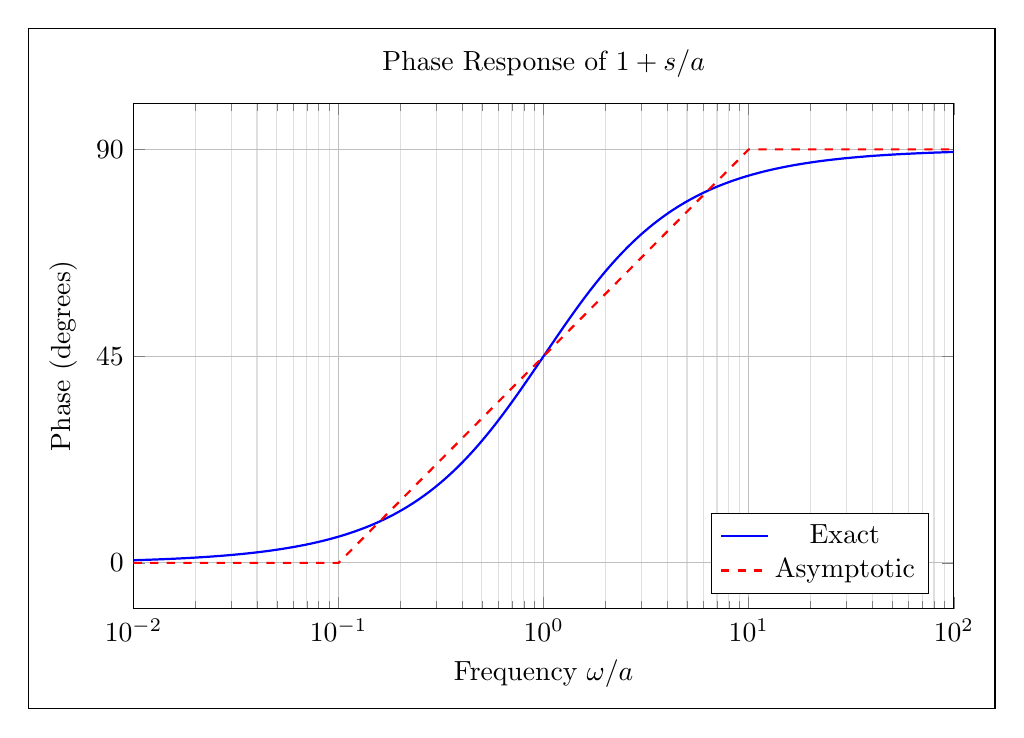
\begin{tikzpicture}[show background rectangle]
    \begin{semilogxaxis}[
        width=12cm, height=8cm,
        title={Phase Response of $1 + s/a$},
        xlabel={Frequency $\omega/a$},
        ylabel={Phase (degrees)},
        grid=both,
        xmin=0.01, xmax=100,
        ymin=-10, ymax=100,
        minor grid style={gray!25},
        major grid style={gray!50},
        legend pos=south east,
        ytick={0, 45, 90},
    ]

    % Exact Phase: atan(x)
    \addplot[blue, thick, domain=0.01:100, samples=300] {atan(x)};
    \addlegendentry{Exact}

    % Asymptotic Phase
    % 0 for x < 0.1
    % 45/dec for 0.1 < x < 10
    % 90 for x > 10
    \addplot[red, dashed, thick] coordinates {
        (0.01, 0) (0.1, 0) (10, 90) (100, 90)
    };
    \addlegendentry{Asymptotic}
    
    \end{semilogxaxis}
\end{tikzpicture}
\end{document}
